\chapter{Análisis de resultados}

\label{Chapter4}

A lo largo del presente capítulo, se analizarán los resultados obtenidos a partir de los experimentos planteados en el
capítulo anterior. Se detallarán las métricas obtenidas, se visualizarán los espacios latentes $\mathbf{z}$ generados
por la parte convolucional de las redes y se analizarán los errores que surgen de aplicar los modelos a los telegramas.

\section{Análisis de métricas}

Los experimentos realizados arrojaron los resultados mostrados en el cuadro \ref{tab:metricas-experimentos}. Las
métricas referidas a la capacidad de clasificación (tasa de acierto, $F_1$) son evaluadas sobre la partición de test
del conjunto de datos de origen donde se conocen las etiquetas a ciencia cierta (MNIST). Por otro lado, las métricas de
adaptación ($MMD$, Dist. $\mathcal{A}$) son evaluadas sobre los espacios latentes que los modelos generaron para las
particiones de test de ambos conjuntos de datos.

Es importante destacar que el mejor modelo es aquel que tiene tanto la mejor capacidad de clasificación como la mejor
adaptación a nuevos conjuntos de datos. Las métricas de clasificación deben ser maximizadas y las de adaptación deben
ser minimizadas.

\begin{table}[H]
    \centering
    \begin{tabular}{cc|rr|rr}
        \toprule
        AD                           & Modelo & Tasa de acierto                     & $F_1$                               & $MMD$                               & Dist. $\mathcal{A}$                 \\
        \midrule
        \multirow[c]{2}{*}{-}        & ResNet & {\footnotesize (2)} 0.9885          & {\footnotesize (2)} 0.9883          & 0.0632                              & 1.9306                              \\
                                     & LeNet  & 0.9811                              & 0.9810                              & 0.0469                              & 1.9515                              \\\hline
        \multirow[c]{2}{*}{DANN}     & ResNet & \textbf{{\footnotesize (1)} 0.9890} & \textbf{{\footnotesize (1)} 0.9890} & 0.1379                              & 1.9776                              \\
                                     & LeNet  & 0.9822                              & 0.9821                              & {\footnotesize (3)} 0.0090          & 1.6774                              \\\hline
        \multirow[c]{2}{*}{ADDA}     & ResNet & 0.9476                              & 0.9485                              & 0.0165                              & 1.8495                              \\
                                     & LeNet  & 0.9191                              & 0.9184                              & 0.0399                              & 1.8495                              \\\hline
        \multirow[c]{2}{*}{DANN+BSP} & ResNet & 0.9780                              & 0.9777                              & 0.0409                              & 1.7888                              \\
                                     & LeNet  & 0.9859                              & 0.9857                              & {\footnotesize (2)} 0.0051          & {\footnotesize (3)} 1.6369          \\\hline
        \multirow[c]{2}{*}{MDD}      & ResNet & {\footnotesize (3)} 0.9864          & {\footnotesize (3)} 0.9863          & 0.0615                              & 1.8987                              \\
                                     & LeNet  & 0.9856                              & 0.9854                              & 0.0399                              & 1.7468                              \\\hline
        \multirow[c]{2}{*}{AFN}      & ResNet & 0.9829                              & 0.9827                              & \textbf{{\footnotesize (1)} 0.0040} & \textbf{{\footnotesize (1)} 1.0886} \\
                                     & LeNet  & 0.9862                              & 0.9859                              & 0.0117                              & {\footnotesize (2)} 1.5747          \\

        \bottomrule
    \end{tabular}
    \caption[Métricas de los experimentos realizados]{Métricas de los experimentos realizados. Entre paréntesis se encuentra la posición que ocupa dentro del top 3 de la columna.}
    \label{tab:metricas-experimentos}
\end{table}

Según los resultados presentados en la tabla anterior, se puede concluir que los modelos entrenados con DANN muestran
un desempeño ligeramente superior en términos de tasa de acierto y $F_1$ en comparación con los modelos baseline
($0.5\%$ de mejora). Sin embargo, es importante destacar que esta diferencia en el rendimiento puede no ser
significativa, por lo que puede considerarse prácticamente nula.

El modelo ResNet18, utilizando AFN, demuestra ser el modelo que combina mejor las métricas de clasificación y
adaptación. A pesar de esto, se destaca que los modelos LeNet entrenados con DANN y AFN obtuvieron buenas métricas en
general, lo que sugiere que en ocasiones, un modelo más complejo no necesariamente garantiza un mejor rendimiento.

Los modelos se aplicaron a todos los telegramas, y se calculó el promedio de $IoU$ por telegrama utilizando el método
descrito en el capítulo \ref{Chapter3}. Además, se determinó la cantidad promedio de aciertos por telegrama utilizando
las etiquetas transcritas en el centro de cómputo, asumiendo que hay pocos errores en ellas. El cuadro
\ref{tab:iou-cant-aciertos-en-telegramas} muestra el $IoU$ promedio y la cantidad de aciertos promedios obtenidos para
los telegramas de prueba.

\begin{table}[H]
    \centering
    \begin{tabular}{cc|rrr}
        \toprule
        AD                           & Modelo & $IoU$ prom.     & \# aciertos prom. & \% aciertos prom. \\
        \midrule
        \multirow[c]{2}{*}{-}        & ResNet & 0.4494          & 4                 & 22\%              \\
                                     & LeNet  & 0.4715          & 6                 & 33\%              \\\hline
        \multirow[c]{2}{*}{DANN}     & ResNet & 0.6941          & 12                & 67\%              \\
                                     & LeNet  & 0.7024          & 12                & 67\%              \\\hline
        \multirow[c]{2}{*}{ADDA}     & ResNet & 0.6763          & 11                & 61\%              \\
                                     & LeNet  & 0.6406          & 10                & 56\%              \\\hline
        \multirow[c]{2}{*}{DANN+BSP} & LeNet  & 0.6695          & 11                & 61\%              \\
                                     & ResNet & 0.6515          & 11                & 61\%              \\\hline
        \multirow[c]{2}{*}{MDD}      & ResNet & 0.5451          & 8                 & 44\%              \\
                                     & LeNet  & 0.5801          & 9                 & 50\%              \\\hline
        \multirow[c]{2}{*}{AFN}      & ResNet & \textbf{0.7486} & \textbf{13}       & \textbf{72\%}     \\
                                     & LeNet  & 0.6493          & 11                & 61\%              \\
        \bottomrule
    \end{tabular}
    \caption[IoU y aciertos por modelo]{IoU promedio y cantidad promedio de aciertos por telegrama obtenidos al aplicar los modelos a los telegramas.}
    \label{tab:iou-cant-aciertos-en-telegramas}
\end{table}

Analizando el cuadro anterior, se confirma la elección del mejor modelo ResNet18 con AFN. Es importante destacar que
independientemente de la técnica de adaptación utilizada, todos los modelos presentan tasas de acierto marcadamente
superiores que aquellos modelos entrenados únicamente con MNIST. Esto sugiere que la adaptación de dominio es
fundamental para obtener un mejor rendimiento en la tarea de clasificación de telegramas. Los modelos entrenados con
técnicas de adaptación logran generalizar mejor y son más efectivos en la tarea de reconocimiento de los patrones
presentes en los telegramas, incluso en presencia de ruido y variaciones en los datos de entrada. Las figuras
\ref{fig:aciertos-lenet} y \ref{fig:aciertos-resnet} muestran la distribución de aciertos por telegrama obtenida
utilizando el modelo baseline y el mejor resultante para LeNet5 y ResNet18 respectivamente.

\begin{figure}[H]
    \centering
    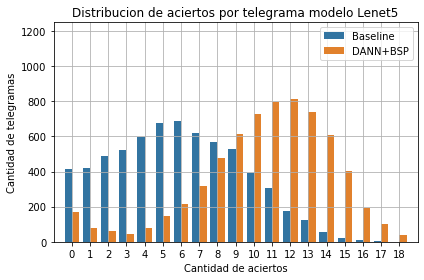
\includegraphics[width=0.7\textwidth]{chapter4/aciertos-lenet.png}
    \caption[Distribución de cantidad de aciertos por telegrama por LeNet5]{Distribución de cantidad de aciertos por telegrama utilizando el modelo baseline (sin adaptación de dominio) y la mejor técnica de adaptación de dominio obtenida para LeNet5.}
    \label{fig:aciertos-lenet}
\end{figure}

\begin{figure}[H]
    \centering
    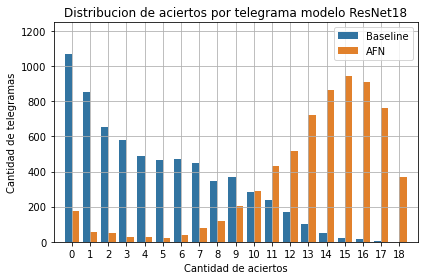
\includegraphics[width=0.7\textwidth]{chapter4/aciertos-resnet.png}
    \caption[Distribución de cantidad de aciertos por telegrama por ResNet18]{Distribución de cantidad de aciertos por telegrama utilizando el modelo baseline (sin adaptación de dominio) y la mejor técnica de adaptación de dominio obtenida para ResNet18.}
    \label{fig:aciertos-resnet}
\end{figure}

Otro punto a resaltar es que cuando no se utiliza adaptación de dominio en la ResNet18, la cantidad de aciertos
promedio por telegrama es incluso peor que la de LeNet5. Esto puede deberse a que, al ser una red mucho más grande y
con más capacidad de aprendizaje, sobreajusta al MNIST no pudiendo generalizar al TDS.

\section{Análisis de los espacios latentes}

Una forma común de visualizar los espacios latentes generados es mediante una técnica de reducción de dimensionalidad,
como Aproximación y Proyección Uniforme de Variedad {\it UMAP} \parencite{mcinnes2018umap}. Es una técnica no lineal que se utiliza para visualizar estructuras de datos complejas en un
espacio de menor dimensión. Al visualizar los espacios latentes utilizando UMAP, se pueden observar patrones y
relaciones en los datos que de otra manera serían difíciles de detectar. Al comparar las distribuciones de los espacios
latentes generados por un modelo para diferentes conjuntos de datos, se pueden identificar las similitudes y
diferencias entre los dominios, lo que puede ser útil para evaluar la capacidad de adaptación de dominio del modelo. En
las siguientes subsecciones se analizarán las representaciones UMAP de los espacios latentes obtenidos por cada modelo
entrenado.

\newpage
\subsection{LeNet}

La figura \ref{fig:umaps-lenet} a continuación contiene las representaciones UMAP obtenidas de los espacios latentes
generados por todos los modelos LeNet.

\begin{figure}[H]
    \centering
    \begin{subfigure}[h]{0.40\textwidth}
        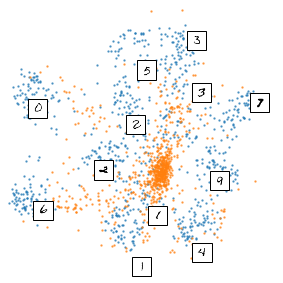
\includegraphics[height=1\textwidth]{chapter4/umap-lenet-so.png}
        \caption{LeNet entrenada con MNIST.}
        \label{fig:umap-lenet-so}
    \end{subfigure}
    \hfill
    \begin{subfigure}[h]{0.40\textwidth}
        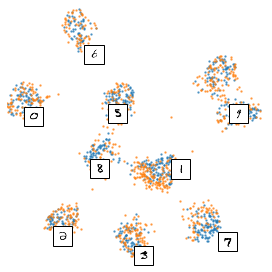
\includegraphics[height=1\textwidth]{chapter4/umap-lenet-dann.png}
        \caption{LeNet entrenada mediante DANN.}
        \label{fig:umap-lenet-dann}
    \end{subfigure}
    \hfill
    \begin{subfigure}[h]{0.40\textwidth}
        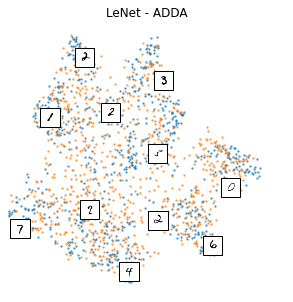
\includegraphics[height=1\textwidth]{chapter4/umap-lenet-adda.png}
        \caption{LeNet entrenada mediante ADDA.}
        \label{fig:umap-lenet-adda}
    \end{subfigure}
    \hfill
    \begin{subfigure}[h]{0.40\textwidth}
        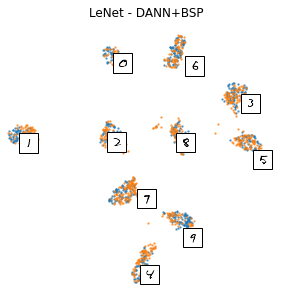
\includegraphics[height=1\textwidth]{chapter4/umap-lenet-bsp.png}
        \caption{LeNet entrenada mediante DANN+BSP.}
        \label{fig:umap-lenet-bsp}
    \end{subfigure}
    \hfill
    \begin{subfigure}[h]{0.40\textwidth}
        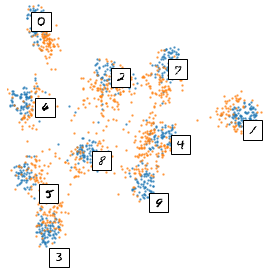
\includegraphics[height=1\textwidth]{chapter4/umap-lenet-mdd.png}
        \caption{LeNet entrenada mediante MDD.}
        \label{fig:umap-lenet-mdd}
    \end{subfigure}
    \hfill
    \begin{subfigure}[h]{0.40\textwidth}
        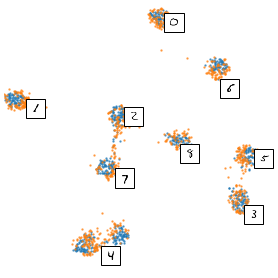
\includegraphics[height=1\textwidth]{chapter4/umap-lenet-afn.png}
        \caption{LeNet entrenada mediante AFN.}
        \label{fig:umap-lenet-afn}
    \end{subfigure}

    \caption[Representación UMAP de las características aprendidas de los modelos LeNet5]{Representación UMAP de las características aprendidas de los modelos LeNet5. Los puntos azules representan observaciones de MNIST y los naranjas de TDS. Los carteles con dígitos son visualizaciones de muestras aleatorias extraídas del conjunto de datos MNIST, lo que permite comprender su ubicación en la representación UMAP.}
    \label{fig:umaps-lenet}
\end{figure}

Se pueden observar los siguientes resultados:

\begin{itemize}
    \item Entrenar el modelo solo con MNIST no permite una buena generalización para TDS, como se muestra en la figura
          \ref{fig:umap-lenet-so}.
    \item Con el entrenamiento mediante ADDA o MDD se comienzan a generar agrupaciones en MNIST, pero no logran generarse de la
          misma manera en TDS, como se puede apreciar en las figuras \ref{fig:umap-lenet-adda} y \ref{fig:umap-lenet-mdd}.
    \item Al entrenar el modelo mediante DANN, se generan agrupaciones similares para ambos conjuntos de datos, como se muestra
          en la figura \ref{fig:umap-lenet-dann}.
    \item Finalmente, al utilizar la técnica de entrenamiento DANN con penalización BSP y AFN, se generan agrupaciones similares
          y más densas para ambos conjuntos de datos, tal como se muestra en las figuras \ref{fig:umap-lenet-bsp} y
          \ref{fig:umap-lenet-afn}.
\end{itemize}

En conclusión, se puede afirmar que la técnica de adaptación de dominio utilizada tiene un gran impacto en el
rendimiento de un modelo LeNet debido a su estructura simple. Entre las diferentes técnicas evaluadas, se puede
observar que DANN+BSP y AFN son las que proporcionan una mejor capacidad de adaptación al modelo LeNet. En general,
estos resultados resaltan la importancia de seleccionar cuidadosamente la técnica de adaptación de dominio adecuada
para un modelo dado a fin de lograr un rendimiento óptimo en diferentes escenarios de aplicación.

\newpage
\subsection{ResNet}

La figura \ref{fig:umaps-resnet} a continuación contiene las representaciones UMAP obtenidas de los espacios latentes
generados por todos los modelos ResNet.

\begin{figure}[H]
    \centering
    \begin{subfigure}[h]{0.39\textwidth}
        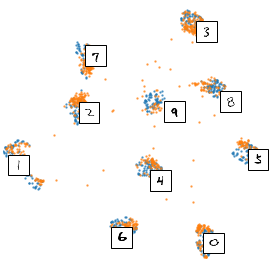
\includegraphics[height=1\textwidth]{chapter4/umap-resnet-so.png}
        \caption{ResNet entrenada con MNIST.}
        \label{fig:umap-resnet-so}
    \end{subfigure}
    \hfill
    \begin{subfigure}[h]{0.39\textwidth}
        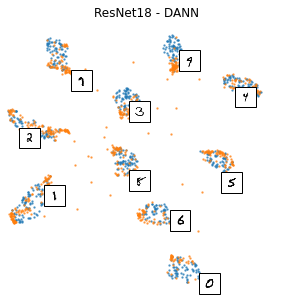
\includegraphics[height=1\textwidth]{chapter4/umap-resnet-dann.png}
        \caption{ResNet entrenada mediante DANN.}
        \label{fig:umap-resnet-dann}
    \end{subfigure}
    \hfill
    \begin{subfigure}[h]{0.39\textwidth}
        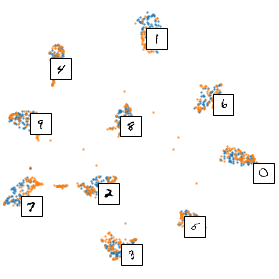
\includegraphics[height=1\textwidth]{chapter4/umap-resnet-adda.png}
        \caption{ResNet entrenada mediante ADDA.}
        \label{fig:umap-resnet-adda}
    \end{subfigure}
    \hfill
    \begin{subfigure}[h]{0.39\textwidth}
        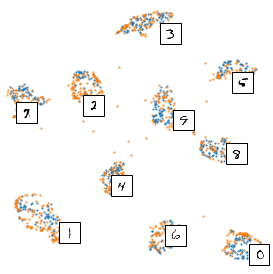
\includegraphics[height=1\textwidth]{chapter4/umap-resnet-bsp.png}
        \caption{ResNet entrenada mediante DANN+BSP.}
        \label{fig:umap-resnet-bsp}
    \end{subfigure}
    \hfill
    \begin{subfigure}[h]{0.39\textwidth}
        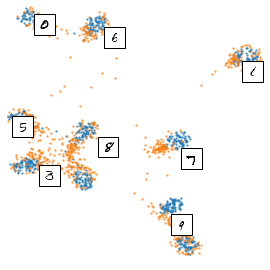
\includegraphics[height=1\textwidth]{chapter4/umap-resnet-mdd.png}
        \caption{ResNet entrenada mediante MDD.}
        \label{fig:umap-resnet-mdd}
    \end{subfigure}
    \hfill
    \begin{subfigure}[h]{0.39\textwidth}
        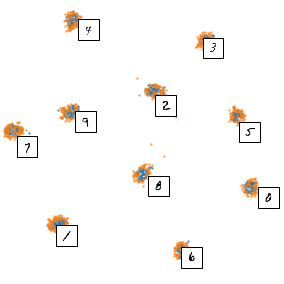
\includegraphics[height=1\textwidth]{chapter4/umap-resnet-afn.png}
        \caption{ResNet entrenada mediante AFN.}
        \label{fig:umap-resnet-afn}
    \end{subfigure}

    \caption[Representación UMAP de las características aprendidas de los modelos ResNet18]{Representaciones UMAP de los espacios latentes de los modelos ResNet18. Los puntos azules representan observaciones de TDS y los naranjas de MNIST. Los carteles con dígitos son visualizaciones de muestras aleatorias extraídas del conjunto de datos MNIST, lo que permite comprender su ubicación en la representación UMAP.}
    \label{fig:umaps-resnet}
\end{figure}

Al analizar las representaciones UMAP de los espacios latentes obtenidos por los modelos ResNet, se pueden observar los
siguientes resultados:

\begin{itemize}
    \item En contraste con los modelos LeNet, la ResNet es más eficaz en la extracción de características {\it out of the box},
          lo que le permite generalizar mejor sin necesidad de técnicas de adaptación de dominio (figura
          \ref{fig:umap-resnet-so}).
    \item La aplicación de técnicas de adaptación de dominio como DANN, DANN con penalización BSP y ADDA mejora la capacidad de
          generalización, pero no de forma significativa en comparación con las mejoras obtenidas con LeNet (figuras
          \ref{fig:umap-resnet-dann}, \ref{fig:umap-resnet-bsp} y \ref{fig:umap-resnet-adda}).
    \item El uso de MDD parece disminuir la capacidad de generalización (figura \ref{fig:umap-resnet-mdd}).
    \item La aplicación de AFN potencia la generalización de la ResNet, obteniendo representaciones de los espacios latentes
          prácticamente idénticas para ambos conjuntos de datos (figura \ref{fig:umap-resnet-afn}).
\end{itemize}

En general, estas representaciones permiten visualizar los resultados obtenidos a partir de las métricas de adaptación
descritas en el cuadro \ref{tab:metricas-experimentos} de la sección anterior.

\section{Análisis de errores}

Los errores de predicción de los modelos pueden ser analizados mediante los histogramas de la métrica $IoU$ que se
obtienen de aplicar los modelos a los telegramas.

\begin{figure}[H]
    \centering
    \begin{subfigure}[h]{0.40\textwidth}
        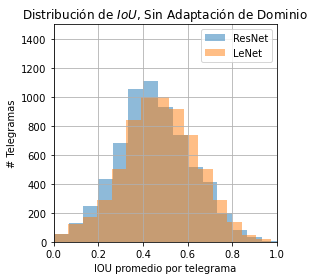
\includegraphics[height=1\textwidth]{chapter4/hist-iou-sin-da.png}
    \end{subfigure}
    \hfill
    \begin{subfigure}[h]{0.40\textwidth}
        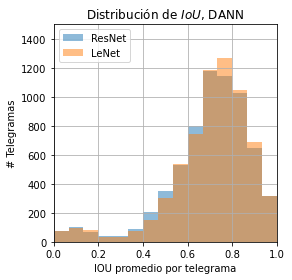
\includegraphics[height=1\textwidth]{chapter4/hist-iou-dann.png}
    \end{subfigure}
    \hfill
    \begin{subfigure}[h]{0.40\textwidth}
        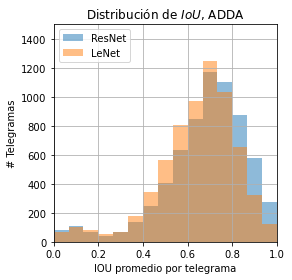
\includegraphics[height=1\textwidth]{chapter4/hist-iou-adda.png}
    \end{subfigure}
    \hfill
    \begin{subfigure}[h]{0.40\textwidth}
        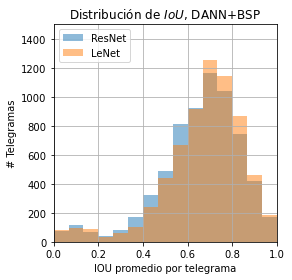
\includegraphics[height=1\textwidth]{chapter4/hist-iou-bsp.png}
    \end{subfigure}
    \hfill
    \begin{subfigure}[h]{0.40\textwidth}
        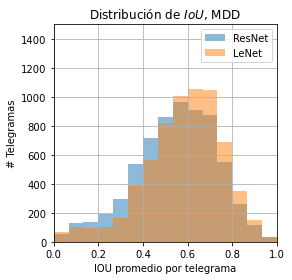
\includegraphics[height=1\textwidth]{chapter4/hist-iou-mdd.png}
    \end{subfigure}
    \hfill
    \begin{subfigure}[h]{0.40\textwidth}
        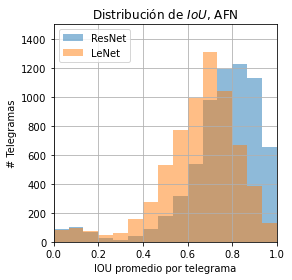
\includegraphics[height=1\textwidth]{chapter4/hist-iou-afn.png}
    \end{subfigure}

    \caption[Histogramas de IoU por modelo]{Histogramas de la métrica $IoU$ promedio por telegrama por cada técnica AD y modelo.}
    \label{fig:histogramas-ious}
\end{figure}

Resulta interesante mencionar existen telegramas que son más difíciles de analizar que otros. Esto puede evidenciarse
en los histogramas de la figura \ref{fig:histogramas-ious} donde se pueden observar un conjunto de observaciones que
contienen valores entre [0, 0.2] en todos los experimentos realizados. Luego de analizar cada uno de estos casos, se
detectaron las siguientes situaciones:

\begin{itemize}
    \item Telegramas cargados de forma errónea: ver ejemplo en el anexo \ref{anexo:telegrama-erroneo}. Hay telegramas que
          corresponden a concejales locales en vez de legisladores nacionales.
    \item Telegramas correctos, pero por alguna cuestión la lógica de extracción de dígitos no funciona correctamente: ver
          ejemplo en el anexo \ref{anexo:telegrama-numeros-juntos}. Los dígitos están unidos sin dejar espacio entre ellos, lo
          que dificulta segmentarlos.
    \item Telegramas donde existen otros caracteres distintos a números: al ser un cuadro de texto libre sin formato, los jefes
          de mesa pueden escribir lo que deseen. Ver ejemplo en el anexo \ref{anexo:telegrama-erroneo-caracteres-especiales}
          donde se representa el $0$ a la izquierda con $X$.
    \item Telegramas de mesas donde la mayor cantidad de votos se las lleva un único partido y completan los votos a la izquierda
          con $0$: al agregar los ceros a la izquierda, aumenta la probabilidad de que el modelo se equivoque con esos ceros que
          no aportan al número final. Ver ejemplo en el anexo \ref{anexo:telegrama-erroneo-muchos-ceros}.
\end{itemize}

En los primeros dos puntos se describen problemas que fueron detectados en el proceso de ETL del capítulo
\ref{Chapter3}. Estandarizar los telegramas agregando un casillero por cada dígito junto a mejorar el proceso de
extracción de los mismos, supondrá una mejora considerable en las capacidades predictivas de los modelos.

El tercer punto presenta un problema dentro de la adaptación de dominio. La misma supone que, si bien los conjuntos de
datos de origen y destino son diferentes, pero representan lo mismo, debe existir la misma cantidad de clases entre
origen y destino. Al agregar uno o varios caracteres adicionales en $TDS$ (como es el ejemplo donde representaban el
$0$ con una $X$), se está incumpliendo este supuesto.

El cuarto punto aumenta la probabilidad de error en los modelos debido a que el $0$ a la izquierda no aporta
significado alguno al número de la cantidad de votos que se desea predecir.

Estandarizar la carga de los telegramas por parte de los jefes de mesa mediante alguna capacitación permitiría reducir
los errores de los puntos tres y cuatro en elecciones futuras.

